\documentclass{jarticle}
\usepackage{amssymb}
\usepackage[dvipdfmx]{graphicx}
\begin{document}


ユーザがアイテムに下した評価スコアを表す評価値行列 $R$ :$m$ $\times$ $n$(ユーザ数×アイテム数。$R$は一般的に、巨大かつ疎な行列である。 $R$ を $U$ :$m$ $\times$ $k$と$V$ :$n$ $\times$ $k$の行列の積で近似することを考える。
(kは潜在因子で人間に理解できる保証はない。)


つまり、

\[
 R \fallingdotseq U V^T (= \hat{R})
\]
と書くことを考える。

\begin{figure}[htbp]
  \begin{center}
  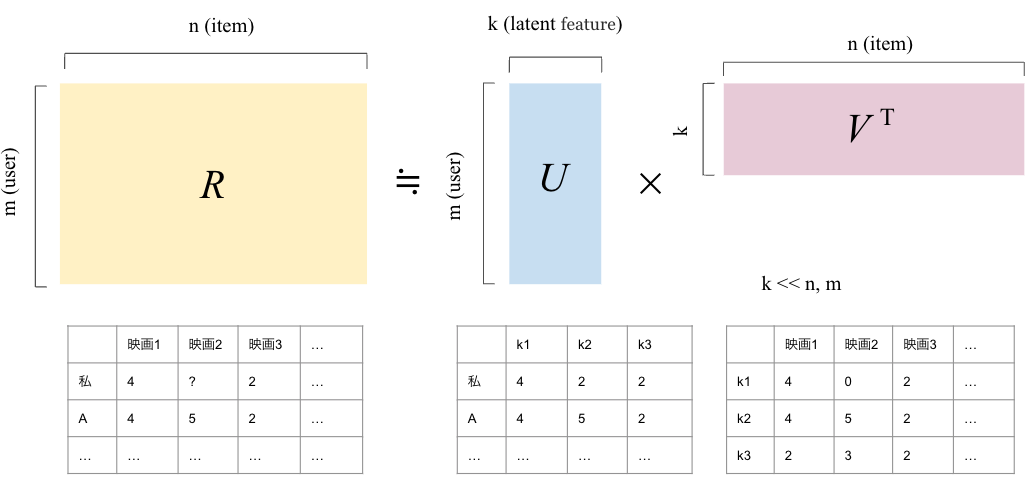
\includegraphics[width=100mm]{matrix_factorization.png}
  \caption{評価値行列の行列分解}
  \end{center}
  \end{figure}
  

この時、推定した評価値行列 $\hat{R} = UV^T$  の $ij$ 成分を $\hat{r}_{ij}$ とすると
\[
 \hat{r}_{ij} =  \sum_{s=1}^{k} u_{is} v_{sj} 
\]
である、ここで

\[
  U = [u_{is}]_{m \times k}
\]
\[
  V = [v_{is}]_{n \times k}
\]
\[
  V^T = [v_{sj}]_{k \times n}
\]
である。

\newpage

以下の目的関数を最小化させる.(単純な2乗誤差)
\[
  J = \frac{1}{2} \sum_{(i,j) \in S} (r_{ij} - \sum_{s=1}^{k} u_{is} v_{sj} )^2
\]

勾配降下法を用いて,
\[
\frac{\partial J}{\partial u_{iq}} = \sum_{j:(i,j) \in S} (r_{ij} - \sum_{s=1}^{k} u_{is} v_{sj} )(-v_{qj}) 
\]

\[
\frac{\partial J}{\partial v_{qj}} = \sum_{i:(i,j) \in S} (r_{ij} - \sum_{s=1}^{k} u_{is} v_{sj} )(-u_{iq}) 
\]

ここで、q = ({1,...,k}) である。
更新式は、

\[
  u_{iq} \longleftarrow u_{iq} - \alpha\left[\frac{\partial J}{\partial u_{iq}}\right]
\]
\[
  v_{qi} \longleftarrow v_{qi} - \alpha\left[\frac{\partial J}{\partial v_{qi}}\right]
\]
ここで、目的関数に正則化項 
\[
  \frac{\lambda_1}{2}\|U\|^2_F + \frac{\lambda_2}{2}\|V\|^2_F
\]
を加えると、目的関数は、
\[
  J = \frac{1}{2} \sum_{(i,j) \in S} (r_{ij} - \sum_{s=1}^{k} u_{is} v_{sj} )^2 + \frac{\lambda_1}{2}\sum_{i=1}^{m}\sum_{s=1}^{k}u_{is}^2 + \frac{\lambda_2}{2}\sum_{s=1}^{k}\sum_{j=1}^{n}v_{sj}^2
\]
勾配は、
\[
\frac{\partial J}{\partial u_{iq}} = \sum_{j:(i,j) \in S} (r_{ij} - \sum_{s=1}^{k} u_{is} v_{sj} )(-v_{qj}) + \lambda_1 u_{iq}
\]
\[
\frac{\partial J}{\partial v_{qj}} = \sum_{i:(i,j) \in S} (r_{ij} - \sum_{s=1}^{k} u_{is} v_{sj} )(-u_{iq}) + \lambda_2 v_{qj}
\]
とかける。(更新式は先ほどと同じ)
\end{document}